\renewcommand{\vec}[1]{\mathbf{#1}}
 \begin{enumerate}


\item First we need to show that a perpendicular from the center of a circle to a chord bisects the chord.\\

Take a circle C of radius $\vec{r}$=2cm, whose center is $\vec{O}$ such that $ \vec{O}$= $\begin{pmatrix}0\\0\end{pmatrix}$. 
$\vec{AB}$ is a chord such that $\vec{OX} \perp \vec{AB}$. We need to show that $\vec{AX}$ = $\vec{BX}$.
\newline
 
\begin{enumerate}
	\item $\triangle OAX \cong \triangle OBX $by RHS rule as: 
	\begin{enumerate}
	\item $\angle{OXA} = \angle{OXB} $ \quad \{90\degree\}
	\item $\vec{OA} = \vec{OB}$ \quad \{radius of the circle\}
	\item $\vec{OX} = \vec{OX}$ \quad \{Common\}
	\end{enumerate}
\end{enumerate}
	Therefore $\vec{AX} = \vec{BX}$\\
	Hence the perpendicular from the center of a circle to a chord bisects the chord.

  
\begin{figure}[!ht]
\centering
\resizebox{\columnwidth}{!}{
\begin{tikzpicture}
[scale=2,>=stealth,point/.style={draw,circle,fill = black,inner sep=0.5pt},]

%Triangle sides
\def\a{5}
\def\b{6}
\def\r{2}
%Coordinates of A
\def\p{1.414}
\def\q{-1.414}
\draw (0,0) circle (2cm);
%Labeling points
\node (A) at (\p,\q)[point,label=below right:$A$] {};
\node (B) at (\p, \p)[point,label=above right:$B$] {};
\node (X) at (\p, 0)[point,label=right:$X$] {};
\node (O) at (0,0)[point,label=left:$O$]{};
%Foot of median

%\node (D) at ($(A)!0.5!(O)$)[point,label=below:$D$] {};
%\node (E) at ($(A)!0.5!(B)$)[point,label=left:$E$] {};
%\node (F) at ($(C)!0.5!(A)$)[point,label=right:$F$] {};

%Drawing triangle ABC
\draw (A) --  (B) -- node[above] {$\textrm{r}$} (O) -- node[below] {$\textrm{r}$} (A);
\draw (X)-- (O);
%Drawing medians BE and CF
%\draw (D) -- (E);
%\draw (D) -- (F);
%\draw (O) -- (B);
%\draw (O) -- (C);
%Drawing EF
%\draw (E) -- (F);

%Labeling sides
%\node [right] at ($(A)!0.5!(E)$) {$\frac{b}{2}$};
%\node [right] at ($(C)!0.5!(E)$) {$\frac{b}{2}$};
%\node [left] at ($(B)!0.5!(F)$) {$\frac{c}{2}$};
%\node [left] at ($(A)!0.5!(F)$) {$\frac{c}{2}$};

%Angles
\tkzMarkRightAngle[fill=green!60,size=.27](O,X,B)
\tkzMarkRightAngle[fill=yellow!60,size=.27](O,X,A)
%\tkzMarkAngle[fill=green!60,size=.3](O,B,A)
%
%\tkzMarkAngle[fill=red!60,size=.7](A,F,D)
%\tkzMarkAngle[fill=red!60,size=.7](A,C,O)
%%
%\tkzMarkAngle[fill=yellow!60,size=.2](A,D,E)
%\tkzMarkAngle[fill=yellow!60,size=.2](A,O,B)
%%
%\tkzMarkAngle[fill=orange!60,size=.2](F,D,A)
%\tkzMarkAngle[fill=orange!60,size=.2](C,O,A)
%
%\tkzMarkAngle[fill=blue!60,size=.3](E,A,F)
\end{tikzpicture}
}
\caption{Circle by Latex-Tikz}
\label{fig:stepone}	
\end{figure}
\end{enumerate}




\item Next we need to show that equal chords of a circle are equidistant from the center.\\

Take a circle C of radius $\vec{r}$=2cm, whose center is $\vec{O}$ such that $ \vec{O}$= $\begin{pmatrix}0\\0\end{pmatrix}$. 
$\vec{AB}$ and $\vec{CD}$ are chords such that $\vec{OX} \perp \vec{AB}$ and $\vec{OY} \perp \vec{CD}$. We need to show that $\vec{OX}$ = $\vec{OY}$.
\newline
 

\begin{enumerate}
	
	\item Since $\vec{OX} \perp \vec{AB}$, $\vec{AX} =  \vec{BX} = \frac{\vec{AB}}{2}$ \{perpendicular from the center of a circle to a chord bisects the chord. \}\\
	Similarly $\vec{CY} =  \vec{DY} = \frac{\vec{CY}}{2}$\\
	\item As $\vec{AB} =  \vec{CD}$\\
	$\frac{\vec{AB}}{2} = \frac{\vec{CD}}{2}$\\
	Hence $\vec{AX} =  \vec{CY}$\\
	
	\item In $\triangle AOX$ and $\triangle COY $\\
	
	\begin{enumerate}
	\item $\angle{OXA} = \angle{OYC} $ \quad \{90\degree\}
	\item $\vec{OA} = \vec{OC}$ \quad \{radius of the circle\}
	\item $\vec{AX} = \vec{CY}$ \quad \{Common\}
	\end{enumerate}
	Hence  $\triangle AOX \cong \triangle COY $by RHS rule.\\
	Therefore, $\vec{OX}=\vec{OY}$
\end{enumerate}
	Hence the equal chords of a circle are equidistant from the center.\\

  
\begin{figure}[!ht]
\centering
\resizebox{\columnwidth}{!}{
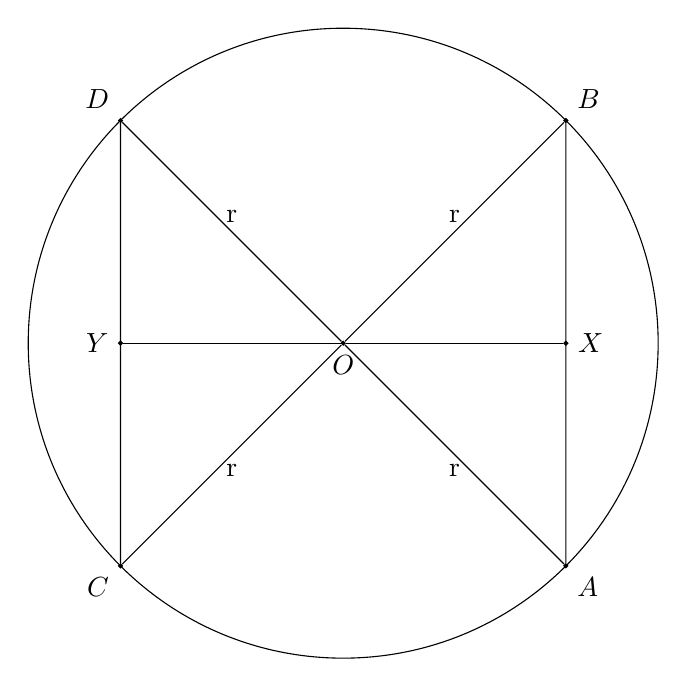
\begin{tikzpicture}
[scale=2,>=stealth,point/.style={draw,circle,fill = black,inner sep=0.5pt},]

%Triangle sides
\def\a{5}
\def\b{6}
\def\r{2}
%Coordinates of A
\def\p{1.414}
\def\q{-1.414}
\draw (0,0) circle (2cm);
%Labeling points
\node (A) at (\p,\q)[point,label=below right:$A$] {};
\node (B) at (\p, \p)[point,label=above right:$B$] {};
\node (X) at (\p, 0)[point,label=right:$X$] {};

\node (C) at (\q,\q)[point,label=below left:$C$] {};
\node (D) at (\q, \p)[point,label=above left:$D$] {};
\node (Y) at (\q, 0)[point,label=left:$Y$] {};

\node (O) at (0,0)[point,label=below:$O$]{};

%Drawing triangle ABC
\draw (A) --  (B) -- node[above] {$\textrm{r}$} (O) -- node[below] {$\textrm{r}$} (A);
\draw (X)-- (O);
\draw (C) --  (D) -- node[above] {$\textrm{r}$} (O) -- node[below] {$\textrm{r}$} (C);
\draw (Y)-- (O);
%Drawing medians BE and CF
%\draw (D) -- (E);
%\draw (D) -- (F);
%\draw (O) -- (B);
%\draw (O) -- (C);
%Drawing EF
%\draw (E) -- (F);

%Labeling sides
%\node [right] at ($(A)!0.5!(E)$) {$\frac{b}{2}$};
%\node [right] at ($(C)!0.5!(E)$) {$\frac{b}{2}$};
%\node [left] at ($(B)!0.5!(F)$) {$\frac{c}{2}$};
%\node [left] at ($(A)!0.5!(F)$) {$\frac{c}{2}$};

%Angles
\tkzMarkRightAngle[fill=green!60,size=.27](O,X,A)
\tkzMarkRightAngle[fill=orange!60,size=.27](O,Y,C)
%\tkzMarkAngle[fill=green!60,size=.3](O,B,A)
%
%\tkzMarkAngle[fill=red!60,size=.7](A,F,D)
%\tkzMarkAngle[fill=red!60,size=.7](A,C,O)
%%
%\tkzMarkAngle[fill=yellow!60,size=.2](A,D,E)
%\tkzMarkAngle[fill=yellow!60,size=.2](A,O,B)
%%
%\tkzMarkAngle[fill=orange!60,size=.2](F,D,A)
%\tkzMarkAngle[fill=orange!60,size=.2](C,O,A)
%
%\tkzMarkAngle[fill=blue!60,size=.3](E,A,F)
\end{tikzpicture}
}
\caption{Circle by Latex-Tikz}
\label{fig:steptwo}	
\end{figure}
\end{enumerate}




